\newcommand{\chapter}[2][]{
	\newcommand{\chapname}{#2}
	\begin{flushleft}
		\begin{minipage}[t]{\linewidth}
			
\includegraphics[height=1cm]{hdht-logo.png}
			\hspace{0pt}	
			\sffamily\bfseries\large Bài  7.
			\begin{flushleft}
				\LARGE\bfseries #1
			\end{flushleft}
		\end{minipage}
	\end{flushleft}
	\vspace{1cm}
	\normalfont\normalsize
}
\chapter[Đồ thị độ dịch chuyển - thời gian \\ Độ dịch chuyển tổng hợp và vận tốc tổng hợp]{Đồ thị độ dịch chuyển - thời gian \\ Độ dịch chuyển tổng hợp và vận tốc tổng hợp}
\section{Lý thuyết}
\subsection{Đồ thị tọa độ - thời gian của chuyển động thẳng đều}
Đồ thị tọa độ - thời gian là đồ thị biểu diễn sự biến đổi \bltext{tọa độ} của vật chuyển động theo \bltext{thời gian}.

Trong chuyển động thẳng đều, đồ thị tọa độ - thời gian có dạng là \bltext{một đường thẳng}.

Ví dụ:
		\begin{center}
	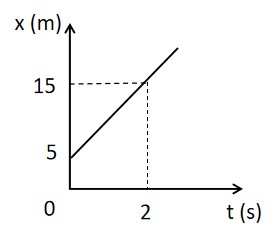
\includegraphics[scale=0.6]{../figs/VN10-PH-03-L-002-4-V2-01.jpg}
\end{center}
\subsection{Tính tương đối của chuyển động}
\vspace*{-1em}
\subsubsection{Quỹ đạo có tính tương đối}
Hình dạng của quỹ đạo của chuyển động trong các hệ quy chiếu khác nhau thì khác nhau. 
\subsubsection{Vận tốc có tính tương đối}
Vận tốc của chuyển động với các hệ quy chiếu khác nhau thì khác nhau. 
\subsection{Hệ quy chiếu đứng yên và hệ quy chiếu chuyển động}
Một chiếc thuyền đang chạy trên một dòng sông. Ta xét chuyển động của thuyền trong hai hệ quy chiếu:
\begin{itemize}
	\item Hệ quy chiếu gắn với bờ (coi như đứng yên) là hệ quy chiếu đứng yên;
	\item Hệ quy chiếu gắn với một vật trôi theo dòng nước là hệ quy chiếu chuyển động.
\end{itemize}

\begin{center}
	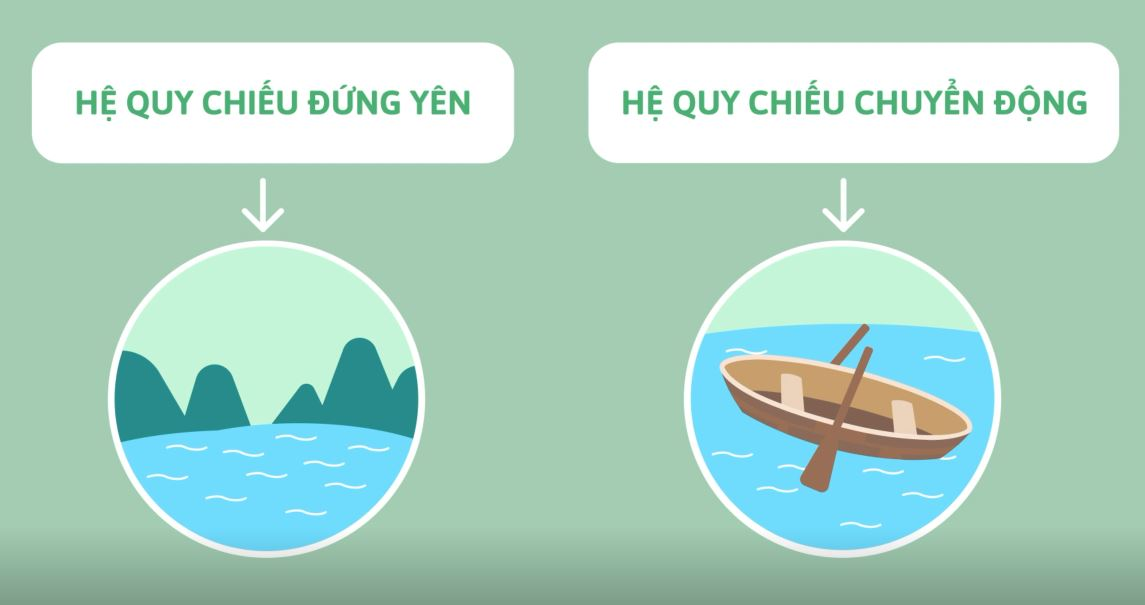
\includegraphics[scale=0.3]{../figs/VN10-PH-07-L-006-2-V2-01.jpg}
\end{center}
\subsection{Công thức cộng vận tốc}
\begin{description}
	\item [Vận tốc tuyệt đối] là vận tốc của vật đối với hệ quy chiếu đứng yên;
	\item [Vận tốc tương đối] là vận tốc của vật đối với hệ quy chiếu chuyển động;
	\item [Vận tốc kéo theo] là vận tốc của hệ quy chiếu chuyển động so với hệ quy chiếu đứng yên.
\end{description}

Vectơ vận tốc tuyệt đối bằng tổng vectơ của vận tốc tương đối và vận tốc kéo theo:
$$\vec{v}_{1,3}=\vec{v}_{1,3}+\vec{v}_{2,3},$$
trong đó:
\begin{itemize}
	\item $\vec{v}_{1,3}$ là vận tốc tuyệt đối;
	\item $\vec{v}_{1,2}$  là vận tốc tương đối;
	\item $\vec{v}_{2,3}$  là vận tốc kéo theo.
\end{itemize}
\section{Mục tiêu bài học - Ví dụ minh họa}
\begin{dang}{Xây dựng đồ thị tọa độ - thời gian,\\ chọn tỉ xích, lập bảng giá trị tương ứng \\cho một vật chuyển động thẳng đều}
	\viduii{2}{Vật chuyển động thẳng đều có đồ thị tọa độ - thời gian như hình vẽ. Phương trình chuyển động của vật có dạng nào sau đây?
		\begin{center}
			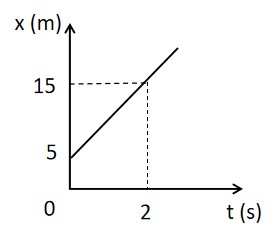
\includegraphics[scale=0.6]{../figs/VN10-PH-03-L-002-4-V2-01.jpg}
		\end{center}
		\begin{mcq}(4)
			\item $x=5+5t$.
			\item $x=4t$.
			\item $x=5-5t$.
			\item $x=5+4t$.
		\end{mcq}
	}
	{	\begin{center}
			\textbf{Hướng dẫn giải}
		\end{center}
		Nhận xét rằng đồ thị mô tả chuyển động của vật đi qua các điểm (\SI{0}{\second},\SI{5}{\meter}) và $(\SI{2}{\second},\SI{15}{\meter})$. Vận tốc của vật được tính từ tọa độ các điểm này 
		\begin{equation*}
			v=\dfrac{x-x_0}{t-t_0}=\dfrac{\SI{15}{\meter}-\SI{5}{\meter}}{\SI{2}{\second}-\SI{0}{\second}}=\SI{5}{\meter/\second}.
		\end{equation*}
		
		Phương trình chuyển động của vật do đó có dạng 
		\begin{equation*}
			x=x_0+vt=5+5t\textrm{ (m, s)}.
		\end{equation*}
		
		\textbf{Đáp án: A}.
	}
	\viduii{3}{	Hai xe chuyển động đều trên cùng một đường thẳng. Vận tốc của xe (I) là $\SI{20}{\meter/\second}$, xe (II) là $\SI{10}{\meter/\second}$. Lúc $t=0$, hai xe cách nhau $\SI{200}{\meter}$. Chọn gốc tọa độ là vị trí của xe (I) lúc $t=0$, chiều dương là chiều chuyển động của hai xe.
		\begin{enumerate}[label=\alph*)]
			\item Viết phương trình chuyển động của mỗi xe.
			\item Vẽ đồ thị chuyển động của hai xe, từ đồ thị hãy xác định thời điểm và nơi gặp nhau của hai xe.
		\end{enumerate}
	}
	{	\begin{center}
			\textbf{Hướng dẫn giải}
		\end{center}
		
		
		\begin{enumerate}[label=\alph*)]
			\item
			Hệ quy chiếu gồm:
			\begin{itemize}
				\item Chiều dương là chiều chuyển động của hai xe;
				\item Gốc tọa độ là vị trí của xe (I) lúc $t=0$;
				\item Mốc thời gian ($t=0$) là lúc hai xe cách nhau $\SI{200}{\meter}$.
			\end{itemize}
			
			Phương trình chuyển động của vật (I) là:
			\begin{equation*}
				x_\text{(I)}=x_{0\text{(I)}} + v_\text{(I)}t =20t\textrm{ (m, s)}.
			\end{equation*}
			
			Phương trình chuyển động của vật (II) là:
			\begin{equation*}
				x_\text{(II)}=x_{0\text{(II)}} + v_\text{(II)}t = 200+10t\textrm{ (m, s)}.
			\end{equation*}
			\item
			Đồ thị chuyển động của hai xe là:
			\begin{center}
				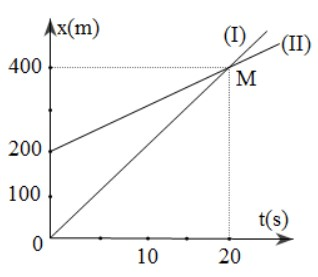
\includegraphics[scale=0.8]{../figs/VN10-PH-03-L-002-4-V2-02.jpg}
			\end{center}
			Hai đồ thị cắt nhau tại M ($t_M=\SI{20}{\second}$, $x_M=\SI{400}{\meter}$). Do đó, nơi gặp cách vị trí xe (I) lúc $t=0$ là $\SI{400}{\meter}$ sau thời gian $\SI{20}{\second}$.
		\end{enumerate}	
	}
\end{dang}
\begin{dang}{Phân biệt được vật chuyển động và đứng yên trong các hệ quy chiếu khác nhau}
	\viduii{3}{Một hành khách ngồi trên toa tàu A, nhìn qua cửa sổ thấy toa tàu B bên cạnh và gạch lát sân ga đều chuyển động như nhau. Nếu lấy vật mốc là nhà ga thì:
		\begin{mcq}
			\item Cả gau tàu đều đứng yên.
			\item Tàu B đứng yên, tàu A chuyển động.
			\item Tàu A đứng yên, tàu B chạy.
			\item Cả hai tàu đều chạy.
		\end{mcq}
		
	}
	{	\begin{center}
			\textbf{Hướng dẫn giải}
		\end{center}
		
		Khi hành khách ngồi trên toa tàu A, mà thấy toa tàu B bên cạnh và gạch lát sân ga đều chuyển động như nhau thì tàu B và sân ga cùng trạng thái chuyển động so với tàu A.
		
		Nếu lấy vật mốc là nhà ga, gạch lát sân ga đứng yên nên tàu B cũng đứng yên. Sân ga chuyển động so với tàu A đồng nghĩa với tàu A chuyển động so với sân ga. 
		
		Vậy trong hệ qui chiếu  gắn với sân ga (lấy vật mốc là nhà ga), tàu A chuyển động, tàu B đứng yên.
		
		
		
		\textbf{Đáp án: B}.
	}
	\viduii{2}{Hành khách 1 đứng trên toa tàu a, nhìn qua cửa số toa sang hành khách 2 ở toa bên cạnh b. Hai toa tàu đang đỗ trên hai đường tàu song song với nhau trong sân ga. Bỗng 1 thấy 2 chuyển động về phía sau. Tình huống nào sau đây chắc chắn không xảy ra?
		\begin{mcq}
			\item Cả hai toa tàu cùng chạy về phía trước. Toa a chạy nhanh hơn toa b.
			\item Cả hai toa tàu cùng chạy về phía trước. Toa b chạy nhanh hơn toa a.
			\item Toa tàu a chạy về phía trước. Toa b đứng yên.
			\item Toa tàu a đứng yên. Toa tàu b chạy về phía sau.
		\end{mcq}
	}
	{	\begin{center}
			\textbf{Hướng dẫn giải}
		\end{center}
		
		Nếu cả hai tàu cùng chạy về phía trước, tàu b chạy nhanh hơn thì hành khách trên  tàu b sẽ chuyển động vượt lên trước hành khách trên tàu a, tức là hành khách 2 sẽ chuyển động về phía trước so với hành khách 1. 
		
		\textbf{Đáp án: B}.
	}
\end{dang}
\begin{dang}{Thực hiện tính vận tốc tuyệt đối,\\ vận tốc tương đối, vận tốc kéo theo}
	\viduii{3}{Một ô tô chạy đều trên một đường thẳng với vận tốc $40\, \textrm{km/h}$. Một ô tô B đuổi theo ô tô A với vận tốc $50\, \textrm{km/h}.$ Xác định vận tốc của:
		\begin{enumerate}[label=\alph*.]
			\item xe ô tô B đối với ô tô A,  
			\item xe ô tô A đối với ô tô B.
		\end{enumerate}
	}
	{	\begin{center}
			\textbf{Hướng dẫn giải}
		\end{center}
		
			Gọi C là một vật đứng yên trên mặt đất trên mặt đất. Hệ quy chiếu gắn với C là hệ qui chiếu đứng yên. Các giá trị vận tốc mà đề bài cho là vận tốc của xe đối với C. 
		
		Trên hình vẽ, ta thể hiện các vectơ vận tốc của các xe A và B đối với C là các vectơ $\vec{v}_{\text{A,C}}$, $\vec{v}_\text{B,C}$.  
		\begin{center}
			\begin{tikzpicture}
				\coordinate (laxis) at (-2,0);
				\coordinate (C) at (0,0);
				\coordinate (A) at (7,0);
				\coordinate (B) at (1,0);
				\coordinate (va) at ($(A)+(2,0)$);
				\coordinate (vb) at ($(B)+(2.5,0)$);
				\coordinate (raxis) at (10,0);
				\draw[->] (laxis) -- (raxis);
				
				
				\draw[->,ultra thick,blue] (A) -- (va);
				\draw[->,ultra thick,green!60!black] (B) -- (vb);
				\node[below=2mm] at (A) {xe A};
				\node[below=2mm] at (B) {xe B};
				\node[below=2mm] at (C) {C};
				\node[right] at (raxis) {$x$};
				\node[above=1mm] at (va) {$\vec{v}_{\text{A,C}}$};
				\node[above=1mm] at (vb) {$\vec{v}_{\text{B,C}}$};
				\coordinate (va2) at ($(A)-(2,0)$);
				\draw[->,ultra thick,red] (A) -- (va2);
				\node[above=1mm] at (va2) {$\vec{v}_{\text{C,A}}$};
				\filldraw (C) circle (4pt);
				\coordinate (vb2) at ($(B)-(2.5,0)$);
				\draw[->,ultra thick,violet] (B) -- (vb2);
				\node[above=1mm] at (vb2) {$\vec{v}_{\text{C,B}}$};
				\foreach \i in {B,A}
				{
					\filldraw (\i) circle (4pt);
				}
			\end{tikzpicture}
		\end{center}
		\begin{enumerate}[label=\alph*.]
			\item Vận tốc của ô tô B đối với ô tô A là: 	$$\vec{v}_{\textrm{B,A}}=\vec{v}_{\textrm{B,C}}+\vec{v}_{\textrm{C,A}},$$
			trong đó, vectơ $\vec{v}_{\textrm{C,A}}$ là vectơ ngược chiều và cùng độ lớn với vectơ $\vec{v}_{\textrm{A,C}}$, thể hiện bằng vectơ màu đỏ như trên hình.
			
			Chiều dương được chọn là chiều chuyển động của hai ô tô.
			Chiếu lên chiều dương, ta được:
			$$v_{\textrm{B,A}}=v_{\textrm{B,C}}+v_{\textrm{C,A}}= 50\, \textrm{km/h}-40\, \textrm{km/h} = 10\, \textrm{km/h}.$$
			\item Vận tốc của ô tô A đối với ô tô B: 	$$\vec{v}_{\textrm{A,B}}=\vec{v}_{\textrm{A,C}}+\vec{v}_{\textrm{C,B}}$$
			trong đó vectơ $\vec{v}_{\textrm{C,B}}$ là vectơ ngược chiều và cùng độ lớn với vectơ $\vec{v}_{\textrm{B,C}}$, thể hiện bằng vectơ màu tím như trên hình.
			
			Chiếu lên chiều dương, ta được:
			$$v_{\textrm{A,B}}=v_{\textrm{A,C}}+v_{\textrm{C,B}}= 40\, \textrm{km/h}-50\, \textrm{km/h} = -10\, \textrm{km/h}.$$
			
			$\bullet$ \textbf{Lưu ý:} Ta cũng có thể suy ra kết quả này từ kết quả câu \textit{a} bằng cách sử dụng công thức 
			$$v_{\textrm{A,B}}=-v_{\textrm{B,A}}=-\SI{10}{\kilo\meter/\hour}.$$
		\end{enumerate}	
	}
	\viduii{3}{Một ô tô chạy đều trên một đường thẳng với vận tốc $40\, \textrm{km/h}$. Một ô tô B chạy theo phương vuông góc với ô tô A có vận tốc $ 30\, \textrm{km/h}.$ Xác định vận tốc của xe ô tô B đối với ô tô A.
	}
	{	\begin{center}
			\textbf{Hướng dẫn giải}
		\end{center}
		
	 	Ta kí hiệu A là ô tô A, B là ô tô B, C là đất. 
	 	Vận tốc của ô tô B đối với ô tô A: 	$$\vec{v}_{\textrm{B,A}}=\vec{v}_{\textrm{B,C}}+\vec{v}_{\textrm{C,A}}.$$
	 	Vectơ $\vec{v}_{\textrm{C,A}}=-\vec{v}_{\textrm{A,C}}$ là vectơ cùng độ lớn nhưng ngược hướng với vectơ $\vec{v}_{\textrm{A,C}}$, được biểu diễn bằng vectơ màu đỏ trong hình. 
	 	\begin{center}
	 		\begin{tikzpicture}[scale=0.8]
	 			\coordinate (laxis) at (0,0);
	 			\coordinate (daxis) at (0,0);
	 			\coordinate (A) at (2,0);
	 			\coordinate (B) at (0,1);
	 			\coordinate (va) at ($(A)+(2,0)$);
	 			\coordinate (vb) at ($(B)+(0,1.5)$);
	 			\coordinate (raxis) at (5,0);
	 			\coordinate (uaxis) at (0,3.5);
	 			\draw[-] (laxis) -- (raxis);
	 			\draw[-] (daxis) -- (uaxis);
	 			\draw[->,ultra thick,blue] (A) -- (va);
	 			\draw[->,ultra thick,green!60!black] (B) -- (vb);
	 			\node[above=2mm] at (A) {xe A};
	 			\node[left=2mm] at (B) {xe B};
	 			%\node[right] at (raxis) {$x$};
	 			%\node[above] at (uaxis) {$y$};
	 			\node[below=1mm] at (va) {$\vec{v}_{\text{A,C}}$};
	 			\node[right=1mm] at (vb) {$\vec{v}_{\text{B,C}}$};
	 			\coordinate (va2) at ($(A)-(2,0)$);
	 			\draw[->,ultra thick,red] (A) -- (va2);
	 			\node[below=1mm] at (va2) {$\vec{v}_{\text{C,A}}$};
	 			\foreach \i in {B,A}
	 			{
	 				\filldraw (\i) circle (2pt);
	 			}
	 			\coordinate (O) at (9,1);
	 			\coordinate (Ou) at ($(O)+(0,1.5)$);
	 			\coordinate (Ol) at ($(O)-(2,0)$);
	 			\coordinate (O2) at ($(O)+(-2,1.5)$);
	 			\draw[->,ultra thick,green!60!black] (O) -- (Ou);
	 			\draw[->,ultra thick,red] (O) -- (Ol);
	 			\draw[dashed] (Ou)--(O2);
	 			\draw[dashed] (Ol)--(O2);
	 			\draw[->,ultra thick,violet] (O)--(O2);
	 			\node[below=1mm] at (Ol) {$\vec{v}_{\text{C,A}}$};
	 			\node[right=1mm] at (Ou) {$\vec{v}_{\text{B,C}}$};
	 			\node[above left] at (O2) {$\vec{v}_{\text{B,A}}$};
	 		\end{tikzpicture}
	 	\end{center}
	 	
	 	Do hai ô tô chuyển động theo hai phương vuông góc nhau nên:
	 	$$v_{\textrm{B,A}}=\sqrt{v_{\textrm{B,C}}^2+v_{\textrm{C,A}}^2}=\sqrt{(\SI{30}{\kilo\meter/\hour})^2+(\SI{40}{\kilo\meter/\hour})^2}=\SI{50}{\kilo\meter/\hour}.$$	
	}
\end{dang}

\begin{dang}{Thực hiện áp dụng công thức cộng vận tốc, tính vận tốc tương đối cùng phương, cùng chiều hoặc ngược chiều với vận tốc kéo theo}
	\viduii{3}{Hai bến sông A  và B cách nhau 11,2 km. Một chiếc ca nô phải mất bao nhiêu thời gian để đi từ A đến B rồi trở lại ngay từ B về A. Biết vận tốc của ca nô so với nước không chảy là $v_1=$ 15 km/h và vận tốc của nước với bờ sông là $v_2=$ 1 km/h.
		
	}
	{	\begin{center}
			\textbf{Hướng dẫn giải}
		\end{center}
		
		Ta gọi $v_{\text{xd}}, v_{\text{nd}}$ lần lượt là vận tốc của thuyền khi nó xuôi dòng và ngược dòng.
		
		Vận tốc của thuyền đối với bờ khi thuyền đi xuôi dòng 
		$$v_{\text{xd}}=v_1+v_2 = \SI{16}{\kilo\meter/\hour}.$$
		Thời gian thuyền đi xuôi dòng khi nó đi từ A đến B
		$$t_{\text{xd}}=\dfrac{AB}{v_{\text{xd}}}=\dfrac{\SI{11.2}{\kilo\meter}}{\SI{16}{\kilo\meter/\hour}}=\SI{0.7}{\hour}.$$
		Vận tốc của thuyền đối với bờ khi thuyền đi ngược dòng 
		$$v_{\text{nd}}=v_1-v_2 = \SI{14}{\kilo\meter/\hour}.$$
		Thời gian thuyền đi ngược dòng khi nó đi từ B đến A
		$$t_{\text{nd}}=\dfrac{AB}{v_{\text{nd}}}=\dfrac{\SI{11.2}{\kilo\meter}}{\SI{14}{\kilo\meter/\hour}}=\SI{0.8}{\hour}.$$
		Tổng thời gian ca nô đi từ A đến B và từ B về A là
		
		$$t= t_{\text{xd}}+ t_{\text{nd}}=\SI{0.7}{\hour}+\SI{0.8}{\hour}=\SI{1.5}{\hour}.$$
	}
	\viduii{3}{Một chiếc thuyền chạy xuôi dòng sông mất 2 giờ để chạy thẳng đều từ bến A ở thượng lưu tới bến B ở hạ lưu và phải mất 3 giờ khi chạy ngược lại từ bến B về đến bến A. Cho rằng vận tốc của thuyền đối với nước là $v_1=$ 30 km/h, vận tốc của dòng nước đối với bờ sông là $v_2$. Tính khoảng cách AB và $v_2$.
	}
	{	\begin{center}
			\textbf{Hướng dẫn giải}
		\end{center}
		
		Ta gọi $v_{\text{xd}}, v_{\text{nd}}$ lần lượt là vận tốc của thuyền khi xuôi dòng và ngược dòng.
		
		Vận tốc của thuyền đối với bờ khi thuyền đi xuôi dòng là:
		$$v_{\text{xd}}=v_1+v_2.$$
		Thời gian thuyền đi xuôi dòng khi nó đi từ A đến B:
		\begin{equation}\label{eq1}
			t_{\text{xd}}=\dfrac{AB}{v_{\text{xd}}}= \dfrac{AB}{v_1+v_2}\quad \Rightarrow\quad \text{AB}=(v_1+v_2)t_{\text{xd}}
		\end{equation}
		Vận tốc của thuyền đối với bờ khi thuyền đi ngược dòng là:
		$$v_{\text{nd}}=v_1-v_2.$$
		Thời gian thuyền đi ngược dòng khi nó đi từ B đến A:
		\begin{equation}\label{eq2}
			t_{\text{nd}}=\dfrac{AB}{v_{\text{nd}}}= \dfrac{AB}{v_1-v_2}\quad\Rightarrow\quad \text{AB}=(v_1-v_2)t_\text{nd}.
		\end{equation}
		Từ hai phương trình \eqref{eq1} và \eqref{eq2}, ta tìm suy ra vận tốc dòng nước và khoảng cách AB:
		\begin{align*}
			(v_1+v_2)t_{\text{xd}}&=(v_1-v_2)t_{\text{nd}}\\
			\quad\Rightarrow\quad	v_2&=\dfrac{\text{nd}-t_\text{xd}}{t_{\text{xd}}+t_\text{nd}}v_1\\
			&=\dfrac{\SI{3}{\hour}-\SI{2}{\hour}}{\SI{2}{\hour}+\SI{3}{\hour}}\times\SI{30}{\kilo\meter/\hour}\\
			&=\SI{6}{\kilo\meter/\hour},\\
			\quad\Rightarrow\quad \text{AB}&=(v_1+v_2)t_\text{xd}\\
			&=(\SI{30}{\kilo\meter/\hour}+\SI{6}{\kilo\meter/\hour})\times\SI{2}{\hour}\\
			&=\SI{72}{\kilo\meter}.
		\end{align*}
	}
\end{dang}